\chapter{决策理论与动态风险}
\label{chap:decision-theory-and-dynamic-risk}

第~\ref{chap:dynamical-systems-and-state-estimation}章说明了给定输入后状态怎样演化，
第~\ref{chap:probability-theory}章则说明给定观测后可以怎样更新结果分布。
但分布本身不会告诉我们应该采取什么行动。即使两个分类器给出完全相同的患病概率，
筛查系统与确诊系统也可能采用不同阈值，因为漏诊和误报的后果不同。决策需要在概率
之外再给出行动集合和损失，并说明怎样汇总随机后果。

当行动还会改变下一时刻的状态时，单步比较又不够。当前多付一点成本，可能换来以后
更好的状态或更有用的信息；当前平均成本较低，也可能隐藏小概率的严重损失。本章由
单步Bayes决策建立“分布加损失”的共同语言，再比较均值、分位数、条件风险价值和
鲁棒目标各自在评价什么。随后把行动放入有限状态的动态过程，从条件期望推导有限时域
与折扣动态规划，并用线性规划对偶连接价值函数和占用流量。

信息价值和动态风险从两个方向扩展这一基准。前者问提前获得一项观测能否改变后续行动，
后者问在每个历史下应怎样评价剩余损失。静态尾部准则、嵌套条件风险和最坏模型递推
可能使用相似的优化式，却不一定定义同一个目标。贯穿本章的判断原则是：先写清随机
对象、可用信息和允许行动，再检查所用风险准则能否与时间递推相容。

\section{把预测分布转化为有代价的行动}
\label{sec:decision-bayes-rules}

\subsection{损失函数、条件风险与Bayes规则}
设观测为\(X\)，未知结果为\(Y\in\mathcal{Y}\)，可选行动属于
\(\mathcal{A}\)。损失函数
\[
  \ell:\mathcal{A}\times\mathcal{Y}\to\mathbb{R}
\]
规定结果为\(y\)时采取行动\(a\)要付出多少代价。给定\(X=x\)以后，结果仍然
不确定，因此需要把每个可能结果的代价按条件概率汇总。
\begin{definition}[条件风险与Bayes决策]
\label{def:decision-conditional-risk-bayes-rule}
给定条件分布核$P(\mathrm dy\mid x)$，假设损失可测，以下出现的期望均有限。各行动的
\term{条件风险}（conditional risk）为
\begin{equation}
  r(a\mid x)
  =
  \mathbb{E}[\ell(a,Y)\mid X=x].
  \label{eq:decision-conditional-risk}
\end{equation}
若条件分布以概率核给出，式~\eqref{eq:decision-conditional-risk}就是
\[
  r(a\mid x)
  =
  \int_{\mathcal{Y}}\ell(a,y)P(\mathrm{d}y\mid x).
\]
有限类别时，积分退化为
\(\sum_y\ell(a,y)p(y\mid x)\)。

在条件风险达到最小值时，任取
\begin{equation}
  a^\star(x)
  \in
  \argmin_{a\in\mathcal{A}}r(a\mid x)
  \label{eq:decision-bayes-action}
\end{equation}
称为一个\term{Bayes行动}（Bayes action），映射
\(\delta^\star:x\mapsto a^\star(x)\)称为\term{Bayes决策规则}
（Bayes decision rule），其中该逐点选择须可测。
\end{definition}
这里的“Bayes”指按照给定条件分布最小化后验期望
损失。条件分布可以来自先验与似然的更新，也可以由其他概率模型给出；Bayes公式负责
更新信念，Bayes规则负责把信念转成行动，两者不是同一步。

若决策规则为\(\delta\)，其总体风险为
\begin{equation}
  R(\delta)
  =
  \mathbb{E}[\ell(\delta(X),Y)].
  \label{eq:decision-rule-risk}
\end{equation}
全期望公式给出
\[
  R(\delta)
  =
  \mathbb{E}\bigl[r(\delta(X)\mid X)\bigr].
\]
因此，只要式~\eqref{eq:decision-bayes-action}中的逐点最小值可测地选取，
\(r(\delta^\star(x)\mid x)\leq r(\delta(x)\mid x)\)便在积分后推出
\(R(\delta^\star)\leq R(\delta)\)。有限行动集合中可按固定次序处理并列，
可测选择没有额外困难；一般行动空间还要核对损失的可测性、下半连续性以及最小值
是否达到。

\begin{example}[有限损失表的逐项计算]
\label{ex:decision-finite-loss-table}
设结果\(Y\in\{y_0,y_1\}\)，两个行动的损失表为
\[
  \begin{array}{c|cc}
    &y_0&y_1\\ \hline
    a_0&0&6\\
    a_1&2&1
  \end{array}
\]
在某个观测\(x\)处，设
\(\mathbb{P}(Y=y_1\mid X=x)=1/4\)。于是
\[
  r(a_0\mid x)
  =
  \frac34\times0+\frac14\times6
  =
  \frac32,
  \qquad
  r(a_1\mid x)
  =
  \frac34\times2+\frac14\times1
  =
  \frac74.
\]
Bayes行动是\(a_0\)，因为它比较的是按条件概率加权后的整行损失，而不是逐列挑选
较小数字。若结果扩展为有限集合\(\{y_1,\ldots,y_m\}\)，同一计算变成
\(r(a\mid x)=\sum_{j=1}^m\ell(a,y_j)
\mathbb{P}(Y=y_j\mid X=x)\)。
\end{example}

这个逐点选择确实给出总体最优，而不只是局部启发式。对任意使用同一观测\(X\)的
可测规则\(\delta\)，塔式法则和逐点最小性依次给出
\begin{align*}
  R(\delta^\star)
  &=
  \mathbb{E}\left[
    \mathbb{E}\{\ell(\delta^\star(X),Y)\mid X\}
  \right]\\
  &=
  \mathbb{E}\left[\min_{a\in\mathcal{A}}r(a\mid X)\right]
  \leq
  \mathbb{E}\left[r(\delta(X)\mid X)\right]
  =
  R(\delta).
\end{align*}
这里要求各项期望存在；有限行动保证可以按固定次序选取第一个最小行动。若
\(\mathcal{A}\)连续，\(\inf_a r(a\mid x)\)可能不达到，逐点最优行动也可能无法
可测地拼成规则，因而不能直接沿用有限集合的结论。

\subsection{代价敏感分类与决策阈值}
考虑二分类\(Y\in\{0,1\}\)与预测行动\(a\in\{0,1\}\)。记
\[
  p(x)=\mathbb{P}(Y=1\mid X=x),
\]
并设正确预测的损失为零，把假阳性的损失记为\(c_{\mathrm{FP}}>0\)，
假阴性的损失记为\(c_{\mathrm{FN}}>0\)。两个行动的条件风险分别为
\begin{align}
  r(1\mid x)
  &=
  c_{\mathrm{FP}}\bigl(1-p(x)\bigr),
  \label{eq:decision-binary-risk-positive}\\
  r(0\mid x)
  &=
  c_{\mathrm{FN}}p(x).
  \label{eq:decision-binary-risk-negative}
\end{align}
选择\(a=1\)当且仅当第一项不大于第二项，即
\begin{equation}
  p(x)
  \geq
  \frac{c_{\mathrm{FP}}}
       {c_{\mathrm{FP}}+c_{\mathrm{FN}}}.
  \label{eq:decision-cost-sensitive-threshold}
\end{equation}
在等号处两个行动风险相同，可以按业务约定处理并列。

若两类错误代价相同，阈值是\(1/2\)。漏诊代价增大时，
式~\eqref{eq:decision-cost-sensitive-threshold}的阈值下降，系统会更愿意
预测阳性。概率模型没有发生变化，变化的是概率进入行动比较的方式。这也说明概率校准
和决策质量不能互相替代：校准良好的\(p(x)\)仍需配合正确损失，错误的损失设定则会把
准确概率转成不合适的行动。

\begin{example}[同一概率对应不同合理行动]
\label{ex:decision-same-probability-different-actions}
设某个样本的阳性概率为\(p(x)=0.3\)。在对称零一损失下，阈值为\(0.5\)，
Bayes行动是预测阴性。若漏诊损失为\(9\)，误报损失为\(1\)，阈值降为
\(1/(1+9)=0.1\)，同一概率对应的Bayes行动改为预测阳性。这个教学数值没有说明
哪组代价适合真实任务；它只展示决策规则还依赖概率之外的价值判断。
\end{example}

图~\ref{fig:decision-cost-thresholds}把条件风险当作概率$p$的函数。
Bayes规则在两条曲线中选择较低者，交点就是阈值。漏诊成本增大后，预测阴性的风险
上升得更快，交点向较小的$p$移动；这使“更谨慎”的含义得到明确解释：谨慎针对哪一种
错误，决定了阈值应向哪个方向改变。

\begin{figure*}[htbp]
  \centering
  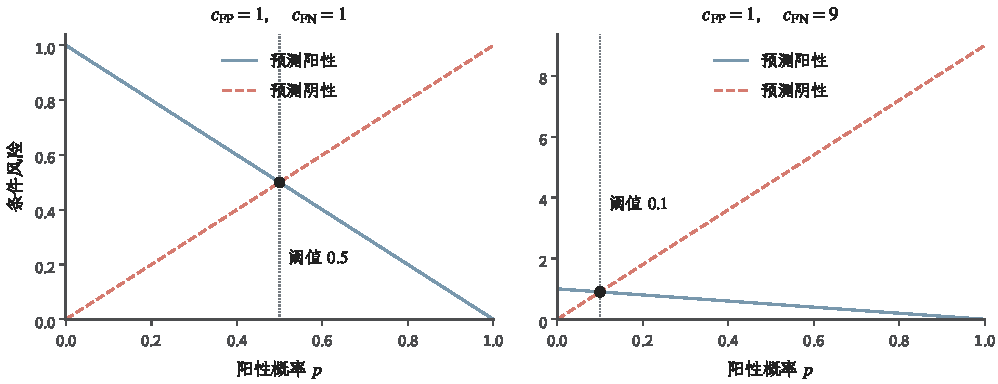
\includegraphics[width=\linewidth]{figures/math-preparation/dynamics/cost-thresholds.pdf}
  \caption{二分类中的条件风险。蓝色实线为预测阳性的风险$c_{\mathrm{FP}}(1-p)$，
  红色虚线为预测阴性的风险$c_{\mathrm{FN}}p$。左图两种错误成本均为$1$，阈值为$0.5$；
  右图仅将漏诊成本增至$9$，阈值降为$0.1$。两图使用相同横轴，纵轴明确显示各自的
  损失范围；教学成本用于说明损失设定如何改变行动。}
  \label{fig:decision-cost-thresholds}
\end{figure*}

\subsection{拒答决策与选择性风险}
模型不确定时，系统可以把样本交给人工复核，而不是被迫给出类别。令类别集合为
\(\{1,\ldots,K\}\)，分类错误使用零一损失，并增加拒答行动
\(\bot\)，其固定损失为\(c_{\mathrm{R}}\in(0,1)\)。若
\[
  p_{\max}(x)=\max_{k}\mathbb{P}(Y=k\mid X=x),
\]
预测最可能类别的条件风险为\(1-p_{\max}(x)\)，拒答风险为
\(c_{\mathrm{R}}\)。因此最优规则为
\begin{equation}
  \delta^\star(x)
  =
  \begin{cases}
    \argmax_k\mathbb{P}(Y=k\mid X=x),
      & p_{\max}(x)\geq1-c_{\mathrm{R}},\\
    \bot,
      & p_{\max}(x)<1-c_{\mathrm{R}}.
  \end{cases}
  \label{eq:decision-reject-rule}
\end{equation}
拒答不是概率模型中的新类别，而是一项具有自身代价的行动。

为描述选择性预测的整体表现，定义\term{覆盖率}（coverage）
\[
  \operatorname{Coverage}(\delta)
  =
  \mathbb{P}\{\delta(X)\neq\bot\},
\]
并在覆盖率为正时定义接受样本上的条件风险
\[
  R_{\mathrm{acc}}(\delta)
  =
  \mathbb{E}\left[
    \ell(\delta(X),Y)
    \,\middle|\,
    \delta(X)\neq\bot
  \right].
\]
低接受风险可以通过拒绝更多样本获得，所以报告它时必须同时报告覆盖率。固定拒答成本
最小化的是包含拒答损失的总体风险，并不等同于在任意指定覆盖率下直接最小化
\(R_{\mathrm{acc}}\)。

若人工复核数量有限，就不能逐个样本独立使用固定
\(c_{\mathrm{R}}\)。例如要求总体接受率至少为\(\kappa\)，可写成
\[
  \min_{\delta}R(\delta)
  \quad\text{s.t.}\quad
  \mathbb{P}\{\delta(X)\neq\bot\}\geq\kappa.
\]
拉格朗日乘子把覆盖预算转成拒答的影子价格，在适当条件下仍得到阈值规则，但阈值由
总体分布和预算共同决定。这类\term{选择性预测}（selective prediction）控制的是
在哪些输入上行动；它不等同于简单提高某个类别的错误代价。

\begin{example}[覆盖预算耦合两个观测点]
\label{ex:decision-two-point-coverage-budget}
设\(X\)等概率取\(x_1,x_2\)，在两个点上作最优分类的条件错误风险分别为
\(0.2\)和\(0.4\)，拒答损失均为\(0.1\)。若逐点比较，两个点都会拒答，因为
\(0.1<0.2<0.4\)，所得覆盖率为零。现在要求
\(\operatorname{Coverage}(\delta)\geq1/2\)，规则至少要接受一个点。接受\(x_1\)并拒答
\(x_2\)的总体风险为
\[
  \frac12\times0.2+\frac12\times0.1=0.15,
\]
反向安排的风险为
\(\frac12\times0.1+\frac12\times0.4=0.25\)。预算把两个观测点的选择联系起来，
最优规则必须联合安排，而不能继续执行原来的逐点拒答。
\end{example}

在有限观测和行动问题中，若允许对每个观测随机选择行动，便可用选择概率作为变量，
把风险与覆盖约束写成线性规划，强对偶给出相应影子价格。若只允许确定性规则，选择
变量带有零一约束，问题一般会变成整数规划，普通线性规划的强对偶不能直接套用。
连续分布或非凸策略类中，拉格朗日形式是否达到原约束问题的值，还要核对可行性、闭性和
相应约束资格；不能仅凭乘子写法断言存在无间隙的阈值解。

\subsection{随机化决策与线性风险}
给定\(x\)，若允许按概率核\(q(\mathrm{d}a\mid x)\)随机选择行动，则条件风险为
\[
  \int_{\mathcal{A}}r(a\mid x)q(\mathrm{d}a\mid x)
  \geq
  \inf_{a\in\mathcal{A}}r(a\mid x).
\]
有限或可数行动集合中，这个积分就是
\(\sum_{a\in\mathcal{A}}q(a\mid x)r(a\mid x)\)。它是各纯行动风险的加权平均，
所以在没有额外耦合约束时，随机化不可能低于纯行动风险的下确界；当最小值达到时，
它至多在多个Bayes行动并列时保持最优。但若不同输入共享总体预算、公平约束或资源约束，
随机化可以精确满足一个纯规则无法达到的平均比例。此时它的作用来自可行域，不是来自
期望损失本身偏好随机行动。

单步Bayes规则由行动、条件分布和损失三者共同确定。接下来保持行动及其随机损失不变，
转而改变汇总随机后果的准则，考察平均损失之外还可以控制什么。

\section{区分平均后果、严重尾部与模型不确定性}
\label{sec:decision-risk-criteria-robustness}

\subsection{期望、方差与风险性质}
本节统一采用“损失越小越好”的方向。设随机损失\(L\)可积。期望
\(\mathbb{E}[L]\)把所有结果按概率线性平均，便于比较和递推，但它可能掩盖稀有而
严重的后果。考虑两个教学方案
\[
  L_{\mathrm{safe}}=1,
  \qquad
  L_{\mathrm{tail}}
  =
  \begin{cases}
    0,&\text{概率 }0.95,\\
    20,&\text{概率 }0.05.
  \end{cases}
\]
两者期望损失都为\(1\)，但第一个方案没有波动，第二个方案把全部平均损失集中到了
最差\(5\%\)的结果中。若任务不能承受这种尾部，单看均值就没有表达完整偏好。

方差\(\operatorname{Var}(L)\)衡量围绕均值的二次波动，均值--方差准则可以写成
\[
  \mathbb{E}[L]+\lambda\operatorname{Var}(L),
  \qquad \lambda\geq0.
\]
它同时惩罚高于和低于均值的偏离；对损失而言，意外变好也会增加方差。此外，方差不是
单调风险准则：即使\(L_1\leq L_2\)逐点成立，较大的\(L_2\)也可能因方差更小而得到
较低的均值--方差值。因此使用它时，应把“波动偏好”和“坏尾部偏好”分开说明。

风险准则的性质说明它怎样响应损失变化。平均损失与尾部损失可以相差很大，但至少应
核对“逐点损失变大，风险会不会反而变小”。以下性质规定的是同一概率空间上损失的比较。
\begin{definition}[相干风险]
\label{def:decision-coherent-risk}
设风险泛函$\rho:L^1(P)\to\mathbb R$。单调性要求对任意$L,L'\in L^1(P)$，
\(L\leq L'\)几乎处处时\(\rho(L)\leq\rho(L')\)；平移等变性要求确定增加
\(m\)单位损失时\(\rho(L+m)=\rho(L)+m\)；凸性要求
\[
  \rho(\tau L+(1-\tau)L')
  \leq
  \tau\rho(L)+(1-\tau)\rho(L'),
  \qquad 0\leq\tau\leq1,
\]
表示按同一场景逐点混合两项损失不会比风险值的同权平均更坏。若再有正齐次性和
次可加性，即$\rho(\lambda L)=\lambda\rho(L)$对$\lambda\geq0$成立，以及
$\rho(L+L')\leq\rho(L)+\rho(L')$，便得到后文使用的\term{相干风险}（coherent risk measure）。
\end{definition}
正齐次与次可加性已经蕴含上述凸性；列出凸性是为了同时说明它与一般凸风险的关系。
这里混合的是同一场景下两项损失的加权和，并非先随机选择某个方案再观察它的损失。
期望满足这些性质。均值--方差准则至少要求
二阶矩存在，并且一般不单调：令\(L_1\)以相同概率取\(0,2\)，令\(L_2=2\)，则
\(L_1\leq L_2\)，但当\(\lambda>1\)时，
\(\mathbb{E}[L_1]+\lambda\operatorname{Var}(L_1)=1+\lambda>2\)，反而把逐点不大的
\(L_1\)评得更差。

\subsection{分位数与风险价值}
\begin{definition}[风险价值]
\label{def:decision-value-at-risk}
对实值随机损失$L$和\(\alpha\in(0,1)\)，其左\(\alpha\)分位数定义为
\begin{equation}
  q_\alpha(L)
  =
  \inf\{z\in\mathbb{R}:\mathbb{P}(L\leq z)\geq\alpha\}.
  \label{eq:decision-loss-quantile}
\end{equation}
在风险管理语境中，同一个量常称为\term{风险价值}
（value at risk, VaR），记作
\(\operatorname{VaR}_{\alpha}(L)=q_\alpha(L)\)。
\end{definition}
它回答“至少\(\alpha\)比例的结果不超过哪一损失水平”。VaR只记录一个切点，
不区分切点以上的损失究竟略高还是极其严重。

在上面的教学例子中，
\[
  \operatorname{VaR}_{0.95}(L_{\mathrm{safe}})=1,
  \qquad
  \operatorname{VaR}_{0.95}(L_{\mathrm{tail}})=0.
\]
按照本书采用的左分位数定义，第二个等式来自
\(\mathbb{P}(L_{\mathrm{tail}}\leq0)=0.95\)。这并不表示尾部方案更安全，
而是表明分位点恰好落在概率质量为\(0.95\)的零损失原子上。离散分布中的边界质量
必须进入尾部计算。

VaR单调且平移等变，却不普遍满足次可加性。设互斥事件\(E_1,E_2\)各有概率
\(0.04\)，令\(L_i=\mathbb{I}\{E_i\}\)。在\(\alpha=0.95\)时，
\(\operatorname{VaR}_{0.95}(L_1)=\operatorname{VaR}_{0.95}(L_2)=0\)，但
\(L_1+L_2\)以概率\(0.08\)取\(1\)，故
\[
  \operatorname{VaR}_{0.95}(L_1+L_2)=1
  >
  \operatorname{VaR}_{0.95}(L_1)
  +
  \operatorname{VaR}_{0.95}(L_2).
\]
两个单独看来未进入最坏\(5\%\)的事件，合并后超过了分位概率预算。这一反例针对
一般分布；在额外分布结构下，VaR仍可能具有更好的性质。

\subsection{条件风险价值与尾部质量}
\term{条件风险价值}（conditional value at risk, CVaR）不只看尾部起点，
还平均最坏的\(1-\alpha\)概率质量\scite{math-rockafellar2000cvar}
\begin{definition}[条件风险价值]
\label{def:decision-conditional-value-at-risk}
对$L\in L^1(P)$和$\alpha\in(0,1)$，定义
\begin{equation}
  \operatorname{CVaR}_{\alpha}(L)
  =
  \inf_{\eta\in\mathbb{R}}
  \left\{
    \eta+
    \frac{1}{1-\alpha}
    \mathbb{E}\bigl[(L-\eta)_+\bigr]
  \right\},
  \qquad
  (u)_+=\max\{u,0\}.
  \label{eq:decision-cvar-optimization}
\end{equation}
\end{definition}
参数\(\eta\)是候选尾部阈值。提高\(\eta\)会直接增加第一项，却会减少超过阈值的
剩余损失；最优点在两种变化之间平衡。

记式~\eqref{eq:decision-cvar-optimization}中花括号内的函数为
\(\phi(\eta)\)。对\(h>0\)，逐点考察正部函数可得
\begin{align*}
  \phi'_+(\eta)
  &=
  1-\frac{\mathbb{P}(L>\eta)}{1-\alpha},\\
  \phi'_-(\eta)
  &=
  1-\frac{\mathbb{P}(L\geq\eta)}{1-\alpha}.
\end{align*}
\(\phi\)是凸函数，所以\(\eta\)最优当且仅当
\[
  \phi'_-(\eta)\leq0\leq\phi'_+(\eta),
\]
也就是
\begin{equation}
  \mathbb{P}(L<\eta)
  \leq\alpha
  \leq
  \mathbb{P}(L\leq\eta).
  \label{eq:decision-cvar-quantile-condition}
\end{equation}
因此任一满足条件的\(\alpha\)分位数都可作为最优阈值。这个推导也解释了为何离散
原子不能直接丢掉：最优阈值处的左右导数可能不同。

令\(q=q_\alpha(L)\)。由
\(\mathbb{P}(L>q)\leq1-\alpha\)及
\(\mathbb{P}(L\geq q)\geq1-\alpha\)，式
\eqref{eq:decision-cvar-optimization}可改写为
\begin{equation}
  \operatorname{CVaR}_{\alpha}(L)
  =
  \frac{
    \mathbb{E}[L\mathbb{I}\{L>q\}]
    +
    q\bigl((1-\alpha)-\mathbb{P}(L>q)\bigr)
  }{1-\alpha}.
  \label{eq:decision-cvar-atomic-tail}
\end{equation}
第二项从\(L=q\)的原子中补足尾部质量。当
\(\mathbb{P}(L\geq q)=1-\alpha\)时，式
\eqref{eq:decision-cvar-atomic-tail}可简写成
\(\mathbb{E}[L\mid L\geq q]\)；分布在\(q\)处连续是保证该等式成立的常见充分条件，
却不是必要条件。无条件使用这个条件期望公式，会在离散分布中平均过多概率质量。

对\(L_{\mathrm{safe}}\)，式~\eqref{eq:decision-cvar-atomic-tail}给出
\(\operatorname{CVaR}_{0.95}=1\)。对\(L_{\mathrm{tail}}\)，最差\(5\%\)
恰好全部位于损失\(20\)，所以
\[
  \operatorname{CVaR}_{0.95}(L_{\mathrm{tail}})=20.
\]
期望看不出两者差异，VaR又在原子边界上给出\(0\)，CVaR则直接反映严重尾部。

\begin{example}[分位点原子中的部分尾部]
  \label{ex:decision-cvar-partial-atom}
  设$L$以概率$0.6,0.3,0.1$分别取$0,2,10$，并取$\alpha=0.75$。
  因为$P(L<2)=0.6<0.75\leq P(L\leq2)=0.9$，分位点为$2$。
  最坏$25\%$由损失$10$的全部$10\%$质量，以及损失$2$的部分$15\%$质量组成，所以
  \[
    \operatorname{CVaR}_{0.75}(L)
    =\frac{0.1\times10+0.15\times2}{0.25}=5.2.
  \]
  直接对事件$L\geq2$条件化会平均$40\%$的质量，得到
  $(0.3\times2+0.1\times10)/0.4=4$，不是此处的CVaR。
  图~\ref{fig:decision-cvar-threshold}同时展示阈值优化式的最低点：阈值前后斜率
  改变，正好对应分位点处需要取部分原子质量。
\end{example}

\begin{figure}[htbp]
  \centering
  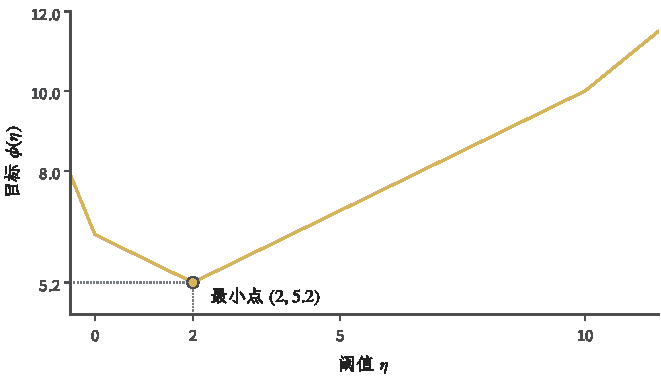
\includegraphics[width=\linewidth]{figures/math-preparation/dynamics/cvar-threshold.pdf}
  \caption{教学损失分布$P(L=0)=0.6$、$P(L=2)=0.3$、$P(L=10)=0.1$在
  $\alpha=0.75$下的阈值目标
  $\phi(\eta)=\eta+4\mathbb E[(L-\eta)_+]$。
  暖黄色折线的最小点为$(2,5.2)$；阈值$2$是VaR，最小目标值$5.2$是CVaR。
  二者位于不同坐标轴，不能把“最优阈值”当作“尾部平均损失”。}
  \label{fig:decision-cvar-threshold}
\end{figure}

\subsection{风险包络与CVaR对偶}
CVaR还有一个对鲁棒决策有用的表达。设\(L\in L^1(P)\)，则
\begin{equation}
  \operatorname{CVaR}_{\alpha}(L)
  =
  \sup_{\zeta}
  \left\{
    \mathbb{E}_P[\zeta L]:
    0\leq\zeta\leq\frac{1}{1-\alpha},\
    \mathbb{E}_P[\zeta]=1
  \right\}.
  \label{eq:decision-cvar-risk-envelope}
\end{equation}
\(\zeta\)是相对于原分布的密度比。上界
\(1/(1-\alpha)\)允许对坏结果加权，却不允许把全部质量压到任意小于
\(1-\alpha\)的事件上。

先看有限分布。对结果\(i\)及原概率\(p_i\)，令
\(q_i=p_i\zeta_i\)。右侧成为线性规划
\[
  \max_{\bm q}\sum_iq_iL_i
  \quad\text{s.t.}\quad
  0\leq q_i\leq\frac{p_i}{1-\alpha},
  \quad\sum_iq_i=1.
\]
最优解从最大损失开始填充允许的概率质量，直到总质量为\(1\)；若最后一个损失值处
只能取部分质量，正好得到式~\eqref{eq:decision-cvar-atomic-tail}中的边界补足。
图~\ref{fig:decision-cvar-reweighting}沿用$L\in\{0,2,10\}$与$\alpha=0.75$的例子，
把名义概率和最坏重加权概率放在同一损失轴上。损失$10$原有质量$0.1$，
至多可以放大到$0.4$；余下$0.6$放在损失$2$，而不是继续把所有质量堆到$10$。
这使密度比上界对应到可直接核对的概率质量。

\begin{figure}[htbp]
  \centering
  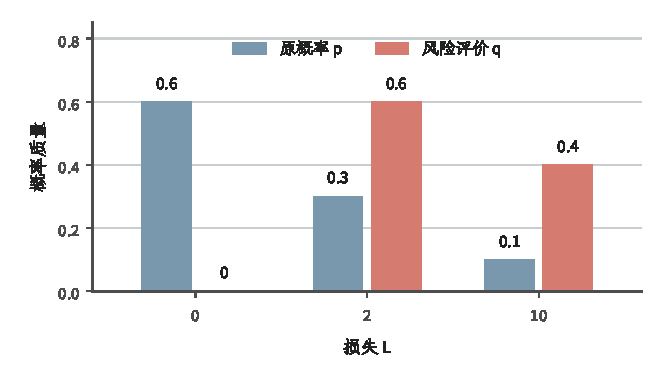
\includegraphics[width=\linewidth]{figures/math-preparation/concept-revision-dynamics/cvar-reweighting.pdf}
  \caption{教学损失$0,2,10$的名义概率为$(0.6,0.3,0.1)$。CVaR$_{0.75}$对偶中的约束
  $q_i\leq4p_i$与$\sum_iq_i=1$给出最优重加权$(0,0.6,0.4)$，
  其期望为$0.6\times2+0.4\times10=5.2$。蓝色为名义质量，红色为对偶最优质量；
  重加权只改变评价权重，不表示真实损失的发生概率已经改变。}
  \label{fig:decision-cvar-reweighting}
\end{figure}

一般表达可由相同的凸对偶关系得到。式~\eqref{eq:decision-cvar-risk-envelope}
说明CVaR是特定风险包络中的最坏期望，但这不意味着任意分布鲁棒目标都等于CVaR。

式~\eqref{eq:decision-cvar-optimization}还可直接验证CVaR的基本性质。若
\(L\leq L'\)，则对每个\(\eta\)都有
\((L-\eta)_+\leq(L'-\eta)_+\)，取下确界得到单调性。把
\(\eta'=\eta-m\)代入\(L+m\)的优化式，得到
\(\operatorname{CVaR}_\alpha(L+m)
=\operatorname{CVaR}_\alpha(L)+m\)。对\(t\geq0\)，令
\(\eta=t\bar\eta\)可得正齐次性；\(t=0\)由归一化单独成立。最后，对任意
\(\eta_1,\eta_2\)，正部函数满足
\[
  \bigl(L_1+L_2-\eta_1-\eta_2\bigr)_+
  \leq
  (L_1-\eta_1)_+
  +
  (L_2-\eta_2)_+.
\]
将这个不等式代入优化表达，并分别对\(\eta_1,\eta_2\)取下确界，得到次可加性。
正齐次性与次可加性又推出凸性。因此，对可积损失，CVaR是单调、平移等变、正齐次且
次可加的相干风险；这些性质不依赖损失分布连续。

\subsection{机会约束、最坏情形与分布鲁棒性}
若要求损失超过阈值\(b\)的概率不能太大，可以使用\term{机会约束}
（chance constraint）
\begin{equation}
  \mathbb{P}(L>b)\leq\varepsilon.
  \label{eq:decision-chance-constraint}
\end{equation}
它控制违规事件的概率，不区分违规后超出阈值多少。条件
\[
  \operatorname{CVaR}_{1-\varepsilon}(L)\leq b
\]
蕴含\(\operatorname{VaR}_{1-\varepsilon}(L)\leq b\)，进而蕴含
式~\eqref{eq:decision-chance-constraint}；这个CVaR替代通常更保守，却同时控制
尾部幅度。反方向一般不成立，因为小概率违规可以具有任意大的损失。

若模型由参数\(\theta\in\Theta\)确定，最坏情形目标
\[
  \inf_a\sup_{\theta\in\Theta}
  \mathbb{E}_{P_\theta}[\ell(a,Y)]
\]
直接比较指定模型集合中的最坏期望。\term{分布鲁棒优化}
（distributionally robust optimization, DRO）则把候选分布放入由距离、矩条件
或散度定义的集合\(\mathcal{P}\)，优化
\[
  \inf_a\sup_{Q\in\mathcal{P}}\mathbb{E}_Q[\ell(a,Y)].
\]
集合如何构造决定保证针对哪些分布；仅把“鲁棒”写进目标名称，不会自动覆盖真实分布。

仍看\(L_{\mathrm{safe}}\)与\(L_{\mathrm{tail}}\)。取事故阈值\(b=10\)和
\(\varepsilon=0.05\)，前者的违规概率为零，后者恰为\(0.05\)，所以两者都满足
机会约束；但二者的\(\operatorname{CVaR}_{0.95}\)分别为\(1\)和\(20\)。若尾部
方案中损失\(20\)的概率并非已知，而只知道\(p\in[0.02,0.08]\)，则其最坏期望为
\(\max_p20p=1.6\)，而机会约束在整个模型集合上并不成立，因为\(p=0.08>0.05\)。
逐路径最坏损失仍是\(20\)。同一有限损失表由此产生了尾部平均、违规概率、最坏期望
和逐路径上界四个不同数值。

在有限样本空间中，若\(\mathcal{P}\)是概率单纯形内的非空闭集，内层期望关于概率
向量线性，紧致性保证最坏分布达到最大值。若集合排除了某些结果，保证也只覆盖其共同
支持；若集合由估计距离球构造，“真实分布落在球内”还需要另行给出抽样置信保证。
交换\(\inf_a\)与\(\sup_Q\)或把内层最大值改写成对偶问题，则还需要凸性、紧致性、
连续性或相应约束资格，不能从有限最大值的存在自动推出。

风险准则、模型扰动与安全约束改变的是三个不同对象。CVaR改变同一损失分布的汇总方式，
最坏模型改变允许的数据生成分布，机会约束限制特定事件概率。它们可以组合，但组合前
必须明确内外层优化次序。下面先回到期望准则，建立行动会改变未来状态时的基准递推。

\section{选择影响未来状态的序贯策略}
\label{sec:decision-dynamic-programming}

静态风险准则评价一个随机后果，却尚未说明当前行动如何改变未来可选后果。
本节先以期望累计损失或奖励为基准，用状态和转移核表达这种影响，
再从条件期望的塔式性质得到Bellman递推。上节的分位数或CVaR不能直接代替递推中的期望；
它们能否跨时间组合，将在条件风险部分单独判断。

\subsection{历史策略与Markov决策过程}
考虑有限时域\(t=0,\ldots,H\)。状态\(S_t\)属于有限集合\(\mathcal{S}\)，
在状态\(s\)可选行动属于非空有限集合\(\mathcal{A}(s)\)。记时刻\(t\)采取行动前的
历史为
\[
  H_t=(S_0,A_0,\ldots,S_t).
\]
采取行动\(a\)后，付出阶段成本\(c_t(s,a)\)，下一状态按转移概率
\[
  P_t(s'\mid s,a)
  =
  \mathbb{P}(S_{t+1}=s'\mid S_t=s,A_t=a)
\]
生成，末端再付出\(c_H(S_H)\)。更具体地，MDP的Markov条件要求，对任一末状态为
\(s\)的历史\(h_t\)，后续转移核满足
\[
  \mathbb{P}(S_{t+1}=s'\mid H_t=h_t,A_t=a)
  =
  P_t(s'\mid s,a).
\]
\begin{definition}[有限Markov决策过程与策略]
\label{def:decision-finite-mdp-policy}
上述有限状态集、各状态的非空有限行动集、初始分布、转移概率、阶段及终端成本
组成有限时域
\term{Markov决策过程}（Markov decision process, MDP）。
一般策略可以根据全部历史随机选择行动，
\(\pi_t(a\mid H_t)\)。若只依赖当前状态，就称为Markov策略；若选择确定行动，
写成\(a=\pi_t(s)\)。
\end{definition}
这里的\(S_t\)承担前章状态\(\bm{x}_t\)的角色，\(A_t\)承担输入
\(\bm{u}_t\)的角色；区别在于本章先使用有限状态与有限行动，并以转移概率取代线性状态
方程。状态必须保留预测未来成本与转移所需的信息。若真实过程还依赖
未记录历史，直接把观测称为“状态”并不会使Markov性质成立\scite{math-puterman1994mdp}

对末状态为\(s\)的一段历史\(h_t\)，一般策略的继续成本应定义为
\begin{equation}
  J_t^\pi(h_t)
  =
  \mathbb{E}_{h_t}^\pi\left[
    \sum_{k=t}^{H-1}c_k(S_k,A_k)+c_H(S_H)
  \right].
  \label{eq:decision-finite-policy-value}
\end{equation}
这里的\(\mathbb{E}_{h_t}^\pi\)表示固定已有历史\(h_t\)，再由策略与转移核生成后续
过程；即使该历史在某个初始分布下概率为零，这个继续过程仍有定义。若\(\pi\)为
Markov策略，Markov条件使\(J_t^\pi(h_t)\)只依赖末状态\(s\)，此时把它记作
\(V_t^\pi(s)\)，并由条件期望得到
\begin{equation}
  V_t^\pi(s)
  =
  \sum_a\pi_t(a\mid s)
  \left[
    c_t(s,a)
    +
    \sum_{s'}P_t(s'\mid s,a)V_{t+1}^\pi(s')
  \right],
  \label{eq:decision-policy-bellman}
\end{equation}
边界条件为\(V_H^\pi(s)=c_H(s)\)。当前成本与未来价值在同一条件期望中相加，
塔式性质负责把后续随机性压缩成\(V_{t+1}^\pi\)。

\subsection{有限时域Bellman递推与策略比较}
由末端向前定义候选最优成本
\begin{align}
  V_H^\star(s)
  &=
  c_H(s),
  \label{eq:decision-finite-bellman-terminal}\\
  V_t^\star(s)
  &=
  \min_{a\in\mathcal{A}(s)}
  \left\{
    c_t(s,a)
    +
    \sum_{s'}P_t(s'\mid s,a)V_{t+1}^\star(s')
  \right\}.
  \label{eq:decision-finite-bellman}
\end{align}

\begin{theorem}[有限时域最优性原理]
\label{thm:decision-finite-horizon-optimality}
在上述有限MDP中，式~\eqref{eq:decision-finite-bellman}给出的
\(V_t^\star(s)\)满足：对每个末状态为\(s\)的历史\(h_t\)，
\[
  V_t^\star(s)=\inf_\pi J_t^\pi(h_t),
\]
其中下确界遍历所有允许的历史依赖随机继续策略。每个时刻和状态选择
式~\eqref{eq:decision-finite-bellman}中任一最小行动，得到的确定性Markov策略最优，
因此有限状态行动下该下确界可以达到。
\end{theorem}

\begin{proof}
证明采用逆向归纳。时刻\(H\)没有行动，结论由
式~\eqref{eq:decision-finite-bellman-terminal}成立。假设对每段末状态为\(s'\)的
历史\(h_{t+1}\)，\(V_{t+1}^\star(s')\)已经等于从该历史继续的最小成本。固定时刻
\(t\)的一段历史\(h_t\)，其末状态为\(s\)。任何策略在该历史下先产生一个行动分布。
给定行动\(a\)和下一状态\(s'\)后，归纳假设说明后续条件期望成本至少为
\(V_{t+1}^\star(s')\)。Markov条件保证下一状态分布为\(P_t(\cdot\mid s,a)\)，
因此该策略从\(h_t\)开始的成本至少为
\[
  \sum_a\pi_t(a\mid h_t)
  \left[
    c_t(s,a)+
    \sum_{s'}P_t(s'\mid s,a)V_{t+1}^\star(s')
  \right].
\]
右侧是各行动括号项的凸组合，不小于其中最小值，也就是
\(V_t^\star(s)\)。

反过来，在当前状态选择达到最小值的行动，并在下一时刻采用归纳假设给出的最优
Markov策略，每一步不等式都取等号，所以能够达到\(V_t^\star(s)\)。由
\(t=H-1,\ldots,0\)归纳，结论成立。
\end{proof}

这个证明同时解释了Markov策略为何足够：在已知模型和期望总成本目标下，历史对未来的
作用已经由当前状态概括。若状态遗漏信息、目标依赖整段轨迹的其他统计量，或策略还受
跨历史预算约束，必须扩充状态或重新证明这一结论。

\begin{example}[两阶段路线选择]
\label{ex:decision-two-stage-route}
初始状态\(s_0\)有“稳妥”和“捷径”两个行动，当前成本都为零。稳妥行动确定进入末端
损失\(2\)的状态；捷径以概率\(0.8\)进入损失\(0\)的状态，以概率\(0.2\)进入
损失\(6\)的状态。末端价值就是末端损失，因此
\[
  Q_0(s_0,\text{稳妥})=2,
  \qquad
  Q_0(s_0,\text{捷径})=0.8\times0+0.2\times6=1.2.
\]
期望成本准则选择捷径。这里没有声称捷径在每条路径上更好；Bellman递推比较的是给定
状态和行动后的条件期望。
\end{example}

同一个路线问题也可以比较不同评价对象，见表~\ref{tab:decision-route-risk-criteria}。
期望递推选捷径，只回答平均损失最小；若要求大损失发生的概率不超过给定预算，任务
就增加了一个不同的约束，必须重新求解。风险偏好是模型的一部分，不能在算完期望最优
以后再把它解释为任意意义下的“最稳妥”。

\begin{table}[htbp]
  \centering
  \begin{tabular}{lcc}
    \toprule
    损失评价 & 稳妥 & 捷径\\
    \midrule
    $\mathbb E[L]$ & $2$ & $1.2$\\
    $P(L>3)$ & $0$ & $0.2$\\
    $\operatorname{VaR}_{0.9}(L)$ & $2$ & $6$\\
    $\operatorname{CVaR}_{0.9}(L)$ & $2$ & $6$\\
    \bottomrule
  \end{tabular}
  \caption{两阶段教学路线在固定分布下的不同指标。捷径以概率$0.8$取损失$0$、
  以概率$0.2$取损失$6$；此处VaR和CVaR同为$6$，是因为最坏$10\%$完全落在
  损失$6$的原子中，不能推广为二者一般相等。}
  \label{tab:decision-route-risk-criteria}
\end{table}

\subsection{折扣Bellman算子与固定点}
现在令转移核\(P\)和有界阶段成本\(c\)不随时间改变，并取折扣因子
\(\gamma\in[0,1)\)。这里的\(\pi\)可以是任意历史依赖随机策略，其价值为
\begin{equation}
  V^\pi(s)
  =
  \mathbb{E}^\pi\left[
    \sum_{t=0}^{\infty}\gamma^t c(S_t,A_t)
    \,\middle|\,S_0=s
  \right].
  \label{eq:decision-discounted-value}
\end{equation}
若\(|c(s,a)|\leq C\)，几何级数保证
\(|V^\pi(s)|\leq C/(1-\gamma)\)。

在有界函数空间上定义Bellman最优算子
\begin{equation}
  (TV)(s)
  =
  \min_{a\in\mathcal{A}(s)}
  \left\{
    c(s,a)+
    \gamma\sum_{s'}P(s'\mid s,a)V(s')
  \right\}.
  \label{eq:decision-discounted-bellman-operator}
\end{equation}
对两组实数\((u_a)\)与\((v_a)\)，有
\[
  \left|\min_a u_a-\min_a v_a\right|
  \leq\max_a|u_a-v_a|.
\]
再利用转移概率非负且和为\(1\)，得到
\begin{align}
  |(TV)(s)-(TW)(s)|
  &\leq
  \gamma\max_a
  \left|
    \sum_{s'}P(s'\mid s,a)
    \bigl(V(s')-W(s')\bigr)
  \right|
  \notag\\
  &\leq
  \gamma\lVert V-W\rVert_\infty.
  \label{eq:decision-bellman-contraction-pointwise}
\end{align}
对\(s\)取最大值得
\begin{equation}
  \lVert TV-TW\rVert_\infty
  \leq
  \gamma\lVert V-W\rVert_\infty.
  \label{eq:decision-bellman-contraction}
\end{equation}

有限状态上的有界函数空间在上确界范数下完备。由第
\ref{thm:analysis-banach-fixed-point}号定理，\(T\)有唯一不动点
\(V^\star\)，价值迭代\(V^{(k+1)}=TV^{(k)}\)从任意有界初值收敛，并满足
\begin{equation}
  \lVert V^{(k)}-V^\star\rVert_\infty
  \leq
  \gamma^k
  \lVert V^{(0)}-V^\star\rVert_\infty.
  \label{eq:decision-value-iteration-error}
\end{equation}
在每个状态选择达到
\(TV^\star=V^\star\)的行动，可得到确定性平稳贪心策略。

为补上最后一步，记该贪心策略为\(\pi^\star\)，并令
\[
  (T_{\pi^\star}V)(s)
  =
  c(s,\pi^\star(s))
  +
  \gamma\sum_{s'}P(s'\mid s,\pi^\star(s))V(s').
\]
与前面的证明相同，\(T_{\pi^\star}\)也是\(\gamma\)压缩，其唯一固定点正是
\(V^{\pi^\star}\)。贪心选择又使
\(T_{\pi^\star}V^\star=TV^\star=V^\star\)，所以固定点唯一性给出
\(V^{\pi^\star}=V^\star\)。这说明Bellman固定点不仅存在，而且确实由一个平稳
确定性策略达到。

还需把这个固定点与所有其他允许策略比较。由
\(V^\star=TV^\star\)，对每个状态行动对都有Bellman不等式
\[
  V^\star(s)
  \leq
  c(s,a)+\gamma\sum_{s'}P(s'\mid s,a)V^\star(s').
\]
沿任意历史依赖随机策略\(\pi\)实际选择的行动逐步条件化，并迭代\(n\)步，得到
\begin{equation}
  V^\star(s)
  \leq
  \mathbb{E}_{s}^{\pi}\left[
    \sum_{t=0}^{n-1}\gamma^t c(S_t,A_t)
    +\gamma^nV^\star(S_n)
  \right].
  \label{eq:decision-discounted-all-policy-comparison}
\end{equation}
\(V^\star\)有界，所以余项的绝对值至多为
\(\gamma^n\lVert V^\star\rVert_\infty\)，随\(n\to\infty\)趋于零；有界成本又保证
折扣成本级数可积。令\(n\to\infty\)便得到
\(V^\star(s)\leq V^\pi(s)\)。结合
\(V^{\pi^\star}=V^\star\)，贪心策略对全部允许的历史依赖随机策略最优。

\(\gamma<1\)同时保证总成本有限并产生严格压缩。若令\(\gamma=1\)，算子通常只能
非扩张，累计成本也可能发散。长期平均成本
\[
  \limsup_{T\to\infty}
  \frac1T
  \mathbb{E}^\pi\left[\sum_{t=0}^{T-1}c(S_t,A_t)\right]
\]
需要平稳性、可达类或单链等额外条件，并常以平均成本\(g\)和相对价值\(h\)满足
\[
  g+h(s)
  =
  \min_a
  \left\{
    c(s,a)+\sum_{s'}P(s'\mid s,a)h(s')
  \right\}.
\]
\(h\)加常数后仍是解，所以不能沿用折扣问题的唯一固定点结论。

有限状态行动使取最小值、可测性和策略选取都较直接。连续状态或行动下，通常还要要求
转移核可测、成本具有适当的下半连续性、可行动作对应非空且具有紧致性或其他强制性，
并用可测选择定理把逐状态最小行动拼成策略。部分可观测时，真实状态不能直接作为策略
输入；只有在滤波信念能概括历史对未来的影响时，才能把信念分布作为新的Markov状态。
这些条件缺失时，形式上的\(\inf\)仍可写出，却未必有达到它的可实施策略。

\subsection{Bellman不等式与占用流量对偶}
有限折扣MDP还能写成线性规划。给定初始分布\(\rho\)，考虑价值端原问题
\begin{equation}
  \begin{aligned}
    \max_{V}\quad&
      (1-\gamma)\sum_s\rho(s)V(s)\\
    \text{s.t.}\quad&
      V(s)
      \leq
      c(s,a)+
      \gamma\sum_{s'}P(s'\mid s,a)V(s'),
      \quad s\in\mathcal{S},\
      a\in\mathcal{A}(s).
  \end{aligned}
  \label{eq:decision-value-lp}
\end{equation}
任一可行\(V\)满足\(V\leq TV\)。反复应用单调的\(T\)，并令迭代收敛到
\(V^\star\)，得到\(V\leq V^\star\)。而\(V^\star=TV^\star\)本身可行，
所以它达到原问题最优值。

为每条Bellman不等式引入乘子\(d(s,a)\geq0\)。拉格朗日函数为
\begin{align*}
  \mathcal{L}(V,d)
  ={}&
  (1-\gamma)\sum_s\rho(s)V(s)\\
  &-
  \sum_{s,a}d(s,a)
  \left[
    V(s)-c(s,a)
    -\gamma\sum_{s'}P(s'\mid s,a)V(s')
  \right].
\end{align*}
收集每个\(V(s)\)的系数。若要使
\(\sup_V\mathcal{L}(V,d)\)有限，必须满足
\begin{equation}
  \sum_a d(s,a)
  =
  (1-\gamma)\rho(s)
  +
  \gamma
  \sum_{\bar s,\bar a}
  P(s\mid\bar s,\bar a)d(\bar s,\bar a),
  \quad s\in\mathcal{S}.
  \label{eq:decision-discounted-flow-conservation}
\end{equation}
此时所有价值系数消失，只剩
\(\sum_{s,a}d(s,a)c(s,a)\)。因此对偶问题为
\begin{equation}
  \begin{aligned}
    \min_{d}\quad&
      \sum_{s,a}d(s,a)c(s,a)\\
    \text{s.t.}\quad&
      \text{式~\eqref{eq:decision-discounted-flow-conservation}},\\
    & d(s,a)\geq0.
  \end{aligned}
  \label{eq:decision-occupancy-lp}
\end{equation}
定理~\ref{thm:opt-lp-strong-duality}保证两个有限LP的最优值相等。

式~\eqref{eq:decision-discounted-flow-conservation}不是抽象代数条件。
\begin{definition}[归一化折扣占用度量]
\label{def:decision-discounted-occupancy}
给定初始分布$\rho$、折扣$0\leq\gamma<1$和策略\(\pi\)，定义归一化折扣
\term{占用度量}（occupancy measure）
\begin{equation}
  d_\pi(s,a)
  =
  (1-\gamma)
  \mathbb{E}_{S_0\sim\rho}^{\pi}
  \left[
    \sum_{t=0}^{\infty}
    \gamma^t
    \mathbb{I}\{S_t=s,A_t=a\}
  \right].
  \label{eq:decision-discounted-occupancy}
\end{equation}
\end{definition}
它把不同时刻访问同一状态行动对的概率相加，近时刻权重大，远时刻权重小。
乘上$1-\gamma$后总质量为$1$；这是一种访问分布，通常不同于Markov链的平稳分布。
把到达状态\(s\)的流量按初始注入和前一步转移分开，正好得到
式~\eqref{eq:decision-discounted-flow-conservation}。逐项写出便是
\begin{align*}
  \sum_a d_\pi(s,a)
  &=
  (1-\gamma)\sum_{t=0}^{\infty}
  \gamma^t\mathbb{P}^{\pi}(S_t=s)\\
  &=
  (1-\gamma)\rho(s)
  +
  \gamma(1-\gamma)
  \sum_{t=0}^{\infty}\gamma^t
  \sum_{\bar s,\bar a}
  \mathbb{P}^{\pi}(S_t=\bar s,A_t=\bar a)
  P(s\mid\bar s,\bar a)\\
  &=
  (1-\gamma)\rho(s)
  +
  \gamma\sum_{\bar s,\bar a}
  P(s\mid\bar s,\bar a)d_\pi(\bar s,\bar a).
\end{align*}
由第一行到第二行时分离\(t=0\)，把其余项的索引前移，再用全概率公式展开下一状态。
对流量方程的状态\(s\)求和，并利用转移概率和为\(1\)，可得
\[
  \sum_{s,a}d_\pi(s,a)=1.
\]
目标值则满足
\begin{equation}
  \sum_{s,a}d_\pi(s,a)c(s,a)
  =
  (1-\gamma)
  \mathbb{E}_{S_0\sim\rho}^{\pi}
  \left[
    \sum_{t=0}^{\infty}\gamma^t c(S_t,A_t)
  \right].
  \label{eq:decision-occupancy-cost}
\end{equation}

反过来，给定任一可行\(d\)，令
\[
  \pi_d(a\mid s)
  =
  \frac{d(s,a)}{\sum_{\bar a}d(s,\bar a)}
\]
用于分母为正的状态；零占用状态上的行动可以任意指定。记
\(x_d(s)=\sum_a d(s,a)\)，并把\(x_d(s)\)与\(\rho(s)\)按状态排列为列向量
\(\bm{x}_d\)与\(\bm{\rho}\)。再令
\(P_{\pi_d}(s'\mid s)=\sum_a\pi_d(a\mid s)P(s'\mid s,a)\)，代入
\(\pi_d\)后，流量方程变成
\[
  \bm{x}_d
  =
  (1-\gamma)\bm{\rho}
  +
  \gamma\bm{P}_{\pi_d}^{\top}\bm{x}_d.
\]
因为\(\gamma<1\)，矩阵
\(\bm{I}-\gamma\bm{P}_{\pi_d}^{\top}\)可由Neumann级数求逆，所以这个固定策略的
折扣状态流量方程只有一个解。策略\(\pi_d\)实际产生的状态占用也满足同一方程，因而
等于\(\bm{x}_d\)，再由
\(d(s,a)=x_d(s)\pi_d(a\mid s)\)恢复同一个状态行动占用度量。由此，价值LP在找满足
所有行动下界的最大价值，流量LP在找可实现的最小成本访问分布。

互补松弛进一步给出
\[
  d^\star(s,a)>0
  \quad\Longrightarrow\quad
  V^\star(s)
  =
  c(s,a)+\gamma\sum_{s'}P(s'\mid s,a)V^\star(s').
\]
最优占用为正的行动必须在对应状态达到Bellman最小值。若采用未乘
\(1-\gamma\)的占用量，流量方程的初始项变为\(\rho\)，总质量变为
\(1/(1-\gamma)\)；两种约定都可使用，但目标与约束必须同步归一化。

上述LP推导依赖有限状态行动、有界成本与\(\gamma<1\)。连续状态下，占用对象是测度，
价值约束是函数不等式；强对偶还需要可测选择、紧致性和适当闭性条件，不能仅把有限求和
替换成积分便宣称结论仍成立。

\section{评价观测能否改善后续行动}
\label{sec:decision-value-of-information}

动态规划在模型和当前信息给定时选择行动。若还可以先观测再行动，
新的问题是观测将怎样改变后续最优决策，以及这项改善是否值得查询成本。
信息价值沿用Bayes风险比较，探索再把获得信息与即时收益放到同一时间过程；
减少熵只在特定目标下代表决策改善。

\subsection{信息价值与观测后决策}
设未知环境参数为\(\Theta\)，当前信息为\(\mathcal{G}\)，相应信念为
\(b(\mathrm{d}\theta)=\mathbb{P}(\Theta\in\mathrm{d}\theta\mid\mathcal{G})\)。
为把重点放在信息如何改变行动，本小节假设行动集合有限，并且各行动的损失可测且可积。
一般行动空间中，下面的点态下确界还须可测，并且需要存在可测的最优或
\(\varepsilon\)-最优选择，才能对应观察后可实施的规则。
若立即选择行动\(a\)，Bayes风险为
\[
  \mathcal{R}(b)
  =
  \inf_a
  \mathbb{E}_{\theta\sim b}[\ell(a,\theta)].
\]
现在可以先观察信号\(Z\)，其条件分布由核
\(K(\mathrm{d}z\mid\theta)\)给出。观察\(Z=z\)后，信念按Bayes规则更新为
\(b_z\)，再选择适合该后验的行动。
\begin{definition}[期望样本信息价值]
\label{def:decision-expected-sample-information-value}
在上述有限行动、可积损失和给定信号核的条件下，信号的\term{期望样本信息价值}
（expected value of sample information, EVSI）定义为
\begin{equation}
  \operatorname{EVSI}(Z\mid b)
  =
  \mathcal{R}(b)
  -
  \mathbb{E}_{Z\mid b}[\mathcal{R}(b_Z)].
  \label{eq:decision-evsi}
\end{equation}
\end{definition}
这是“无信号时的最小风险”减去“看到信号后再行动的平均最小风险”。

EVSI非负。证明不需要熵或互信息，只需注意观察后总可以忽略\(Z\)，继续采用原来的
行动。若无信号风险的下确界由\(a^\star\)达到，则对每个\(z\)，
\[
  \mathcal{R}(b_z)
  \leq
  \mathbb{E}[\ell(a^\star,\Theta)\mid Z=z,\mathcal{G}].
\]
再对\(Z\)取期望并使用塔式性质，得到
\[
  \mathbb{E}_{Z\mid b}[\mathcal{R}(b_Z)]
  \leq
  \mathbb{E}[\ell(a^\star,\Theta)\mid\mathcal{G}]
  =
  \mathcal{R}(b).
\]
在一般行动空间中，若最优行动不达到但存在可测的
\(\varepsilon\)-最优选择，可改取风险不超过
\(\mathcal{R}(b)+\varepsilon\)的行动。相同推导给出观察后平均风险不超过
\(\mathcal{R}(b)+\varepsilon\)，再令\(\varepsilon\downarrow0\)，仍得到EVSI非负。
若取得信号要付成本\(k\)，应比较净价值
\(\operatorname{EVSI}-k\)。免费信息不会降低最优价值，不表示任何有成本的观测都值得
获取。

若能够直接知道\(\Theta\)，得到\term{完全信息价值}
\begin{equation}
  \operatorname{EVPI}(b)
  =
  \inf_a\mathbb{E}_{b}[\ell(a,\Theta)]
  -
  \mathbb{E}_{b}\left[\inf_a\ell(a,\Theta)\right].
  \label{eq:decision-evpi}
\end{equation}
任意样本信号都是\(\Theta\)的随机加工，决策者在知道\(\Theta\)后可以模拟该信号，
所以\(\operatorname{EVSI}\leq\operatorname{EVPI}\)。等号只在信号已经保留当前
决策所需的全部信息时成立。

\begin{example}[辨别信号与无关信号]
\label{ex:decision-informative-and-irrelevant-signals}
沿用二分类决策，设当前阳性概率为\(0.3\)，假阳性损失为\(1\)，假阴性损失为
\(9\)。不观察新信号时，预测阳性的风险为\(0.7\)，预测阴性的风险为\(2.7\)，
故\(\mathcal{R}(b)=0.7\)。若免费信号\(Z_{\mathrm{perf}}\)完全揭示类别，观察后
总能选对，平均风险降为零，因而
\(\operatorname{EVSI}(Z_{\mathrm{perf}}\mid b)=0.7\)。

另取一个与类别独立的公平硬币信号\(Z_{\mathrm{coin}}\)。无论看到哪一面，后验阳性
概率仍为\(0.3\)，最优行动和风险都不变，所以
\(\operatorname{EVSI}(Z_{\mathrm{coin}}\mid b)=0\)。若取得完全信号的成本为
\(0.8\)，其净价值反而为\(-0.1\)。可辨别性、任务价值和扣除成本后的净收益是三个
不同判断。
\end{example}

\subsection{信息量与决策价值的区别}
互信息衡量观察\(Z\)后关于\(\Theta\)的不确定性平均减少多少，信息价值衡量最优
决策损失减少多少。一个信号可以精确揭示与当前行动无关的参数，互信息很大而EVSI为零；
另一个二元信号只在临界阈值附近略微改变信念，却可能翻转高代价行动，EVSI很大。
因此，主动获取信息时必须说明优化的是预测精度、熵减少还是决策价值。

当损失为对数评分且行动本身是预测分布时，信息增益与期望对数损失改善会形成直接联系。
对一般分类代价、资源分配或控制损失，这种等价不再成立。使用熵作为查询代理时，需要
证明它与任务损失之间的关系，不能只因二者都随信息变化便混用。

\subsection{两臂选择中的探索收益}
考虑两轮选择。已知臂每次成功概率为\(0.6\)。未知臂的成功概率
\(\Theta\)只可能是\(0.3\)或\(0.9\)，先验概率各为\(1/2\)。当前未知臂的后验
均值也是\(0.6\)，所以若只看本轮期望收益，两臂并列。

若第一轮选择未知臂，成功的边缘概率为\(0.6\)。观察成功后，
\[
  \mathbb{P}(\Theta=0.9\mid\text{成功})
  =
  \frac{0.9\times0.5}
       {0.9\times0.5+0.3\times0.5}
  =0.75,
\]
下一轮未知臂的后验成功概率为
\(0.75\times0.9+0.25\times0.3=0.75\)。若第一轮失败，
\[
  \mathbb{P}(\Theta=0.9\mid\text{失败})
  =
  \frac{0.1\times0.5}
       {0.1\times0.5+0.7\times0.5}
  =0.125,
\]
未知臂的后验成功概率降为\(0.375\)，下一轮改选已知臂。
因此“先试未知臂，再按结果选择”的两轮期望收益为
\begin{equation}
  0.6+
  0.6\times0.75+
  0.4\times0.6
  =
  1.29.
  \label{eq:decision-two-arm-information-value}
\end{equation}
始终选择已知臂的期望收益为\(1.2\)。多出的\(0.09\)来自第一轮观测改变了第二轮
行动，而不是来自未知臂当前均值更高。

这个例子把\term{探索}（exploration）的核心作用写得很小：某个行动既产生即时结果，
也产生影响后续选择的信息。若只剩一轮，信息没有后续使用机会，两臂又回到并列。若
试验成本上升或先验差异缩小，探索价值也会改变。完整的多臂和强化学习算法还要处理
未知参数估计、长时域规划和计算问题，本节只建立信息进入决策的数学位置。

上述更新假设两轮共享同一个不变参数\(\Theta\)，并且每轮只观察所选臂的结果；
未选臂的反事实结果不可见。若每轮同时观察所有臂，信息结构会改变；若成功概率随时间
漂移而仍按固定\(\Theta\)更新，后验和探索收益的计算都不再对应真实过程。

\subsection{自适应反馈与统计证据}
选择最不确定的样本、反复试验某个行动或在区间足够窄时停止，都会让数据取得规则依赖
过去观测。信息价值说明为何要这样选择，却不自动保证选择后的估计仍然可靠。若希望报告
置信区间或识别最优行动，需要回到
第~\ref{sec:stoch-martingales-stopping-sequential-concentration}节的停时条件和
第~\ref{sec:stoch-self-normalized-adaptive-design}节的可预测设计，核对当前查询是否在
当前噪声揭晓前确定，以及保证是否对全部查看时刻同时成立。

遗憾则使用另一比较口径。令\(Y_t\)为第\(t\)轮观察到的随机奖励，并定义给定环境参数
\(\theta\)时的平均奖励函数。记\(\mathcal{H}_{t-1}\)为第\(t\)轮行动前可用的信息，
要求\(A_t\)在\(Y_t\)揭晓前依据这些信息选定，并假设
\[
  \mathbb{E}\left[
    Y_t
    \,\middle|\,
    \mathcal{H}_{t-1},A_t=a,\Theta=\theta
  \right]
  =
  \mu(a,\theta)
  \quad\text{几乎处处}.
\]
这个条件要求给定环境参数、历史和本轮行动后，奖励均值只由
\((a,\theta)\)决定，使当前奖励噪声在给定本轮行动后仍具有正确的条件均值；自适应选择本身
仍会改变各行动的访问次数和数据的联合分布。同时假设该均值不随
轮次改变。若第\(t\)轮选择\(A_t\)，并取
\[
  a^\star(\theta)
  \in
  \argmax_a\mu(a,\theta),
\]
则以平均奖励比较的累计伪遗憾为
\[
  \operatorname{Reg}_T(\theta)
  =
  \sum_{t=1}^{T}
  \left[
    \mu(a^\star(\theta),\theta)-\mu(A_t,\theta)
  \right].
\]
它在相同环境参数下，把算法所选行动的平均奖励与始终选择最优行动的平均奖励比较。
若算法或\(\Theta\)也是随机的，还可再对
\(\operatorname{Reg}_T(\Theta)\)取期望。直接用实现奖励之差定义的随机遗憾还包含奖励
噪声，不能与上述平均奖励差混为一谈。EVSI衡量一项信息在当前决策问题中的期望价值。
二者相关，却不能用一次信息增益直接替代长期遗憾证明。

\section{让风险评价与逐时获得的信息相容}
\label{sec:decision-dynamic-risk-time-consistency}

本节回到尾部与鲁棒要求，把静态风险准则放进逐时获得信息的决策。
关键不只是风险值能否计算，而是今天认可的计划在明天条件化之后是否仍按同一规则评价。
条件风险映射与嵌套递推规定这种规则，矩形结构则说明最坏模型能否按局部选择拼接。

\subsection{静态CVaR与条件偏好反转}
期望能够递推，是因为塔式性质把未来条件期望再平均回当前期望。若在初始时刻对整段累计
损失一次性计算CVaR，这项性质通常不再成立。下面的两阶段教学例子展示缺口。

初始时以相同概率进入节点\(N\)与节点\(B\)。节点\(N\)的损失固定为\(2\)；
在\(B\)中可以选择固定方案\(F\)或随机方案\(R\)：
\[
  L_F=3.5,
  \qquad
  L_R=
  \begin{cases}
    0,&\text{条件概率 }1/2,\\
    4,&\text{条件概率 }1/2.
  \end{cases}
\]
若初始时承诺在\(B\)选择\(F\)，总损失以概率\(1/2\)取\(2\)，以概率
\(1/2\)取\(3.5\)，所以最坏一半的平均为
\[
  \operatorname{CVaR}_{0.5}(L^{F})=3.5.
\]
若承诺选择\(R\)，无条件损失分别以概率\(1/4,1/2,1/4\)取\(0,2,4\)。
最坏一半的概率质量由全部损失\(4\)和一半的损失\(2\)组成，故
\[
  \operatorname{CVaR}_{0.5}(L^{R})
  =
  \frac{(1/4)\times4+(1/4)\times2}{1/2}
  =3.
\]
初始静态CVaR因此严格偏好承诺\(R\)。

但真正到达\(B\)以后，条件分布已经改变。此时
\[
  \operatorname{CVaR}_{0.5}(L_F\mid B)=3.5,
  \qquad
  \operatorname{CVaR}_{0.5}(L_R\mid B)=4,
\]
决策者会改选\(F\)。初始评价时，节点\(N\)的损失\(2\)占用了静态尾部的一部分；
到达\(B\)后，节点\(N\)已经排除，尾部质量只在\(B\)的条件分布中重新分配。偏好
反转来自条件化改变了排序，不是CVaR计算错误，也不表示所有风险准则都会出现同样
冲突。普通期望仍由塔式法则保持递推。

表~\ref{tab:decision-static-conditional-nested}固定同一两阶段分布，列出三种评价的
差异。静态目标把尾部预算分给整棵树；条件评价先排除未到达的分支；嵌套目标则要求每个
下一节点先给出自己的风险评价值。后者可以递推，却因此改变了最初评价的随机对象。

\begin{table*}[htbp]
  \centering
  \begin{tabularx}{\linewidth}{XccX}
    \toprule
    评价口径 & 承诺$F$ & 承诺$R$ & 比较依据\\
    \midrule
    初始静态$\operatorname{CVaR}_{0.5}$ & $3.5$ & $3$ & 整棵树最坏一半的终端损失\\
    到达$B$后的条件$\operatorname{CVaR}_{0.5}$ & $3.5$ & $4$ & $B$内部最坏一半的损失\\
    两层嵌套$\operatorname{CVaR}_{0.5}$ & $3.5$ & $4$ & 先评价下一节点，再评价节点风险\\
    \bottomrule
  \end{tabularx}
  \caption{同一教学例中的静态、条件和嵌套风险。节点$N$固定损失为$2$，根节点等概率
  到达$N$或$B$。前两行偏好反转；嵌套目标偏好$F$，但它评价的目标与静态总损失CVaR
  不同。第三行的递归定义将在下一小节建立。}
  \label{tab:decision-static-conditional-nested}
\end{table*}

\subsection{条件风险映射与信息适应性}
令
\[
  \mathcal{F}_0\subseteq\mathcal{F}_1\subseteq\cdots
  \subseteq\mathcal{F}_H
\]
表示随历史增长的信息。下一步风险应按当前历史分别评价，而不能允许阈值偷看未来结果。
\begin{definition}[一步条件风险映射]
\label{def:decision-conditional-risk-mapping}
在同一概率空间上，一步\term{条件风险映射}
（conditional risk mapping）
\[
  \rho_t:
  L^\infty(\mathcal{F}_{t+1})
  \longrightarrow
  L^\infty(\mathcal{F}_t)
\]
把下一时刻可知的有界随机损失，转换成当前信息下可比较的风险。映射作用于几乎处处
相等的等价类，因此输出也按几乎处处相等理解。
\end{definition}
常用的两项性质是：
\begin{align}
  Z\leq Z'
  &\Longrightarrow
  \rho_t(Z)\leq\rho_t(Z'),
  &&\text{单调性},
  \label{eq:decision-conditional-risk-monotonicity}\\
  \rho_t(Z+M)
  &=
  \rho_t(Z)+M,
  \quad M\in L^\infty(\mathcal{F}_t),
  &&\text{平移等变性}.
  \label{eq:decision-conditional-risk-translation}
\end{align}
第一项表示逐点更大的未来损失不应得到更低风险；第二项表示当前已经确定的成本可以直接
提出风险映射。通常还约定\(\rho_t(0)=0\)。条件期望
\(\rho_t(Z)=\mathbb{E}[Z\mid\mathcal{F}_t]\)满足这些性质。

条件CVaR可以写成
\begin{equation}
  \operatorname{CVaR}_{\alpha,t}(Z)
  =
  \operatorname*{ess\,inf}_{\eta\in
    L^\infty(\mathcal{F}_t)}
  \left\{
    \eta+
    \frac{1}{1-\alpha}
    \mathbb{E}[(Z-\eta)_+\mid\mathcal{F}_t]
  \right\}.
  \label{eq:decision-conditional-cvar}
\end{equation}
这里阈值\(\eta\)可以依赖当前历史，却不能依赖尚未观察的下一步结果。
本质下确界忽略当前概率为零的历史差异。有限概率树上，它等价于在每个当前节点分别
应用式~\eqref{eq:decision-cvar-optimization}。

\subsection{嵌套动态风险与时间一致性}
\begin{definition}[嵌套动态风险]
\label{def:decision-nested-dynamic-risk}
给定一步条件风险映射$(\rho_t)$，令\(C_t\in L^\infty(\mathcal{F}_t)\)表示时刻\(t\)已经知道的有界阶段损失。
从后向前定义
\begin{align}
  \mathcal{R}_{H}(C_H)
  &=
  C_H,\\
  \mathcal{R}_{t}(C_t,\ldots,C_H)
  &=
  C_t+
  \rho_t\bigl(
    \mathcal{R}_{t+1}(C_{t+1},\ldots,C_H)
  \bigr).
  \label{eq:decision-nested-dynamic-risk}
\end{align}
这称为\term{嵌套动态风险}（nested dynamic risk）。
\end{definition}
当前评价先接受下一时刻对
剩余损失的评价，再用当前条件风险汇总各下一状态。比较两份未来计划时，还需要固定
相同的当前损失，否则当前评价的差异可能来自已经付出的成本。
\begin{definition}[递归意义下的时间一致性]
\label{def:decision-time-consistency}
动态风险族$(\mathcal R_t)$称为具有\term{时间一致性}（time consistency），如果
对每个$t=0,\ldots,H-1$、任意两组从$t+1$开始的有界适应损失，以及同一当前损失$C_t$，只要
$\mathcal R_{t+1}(C_{t+1:H})\leq\mathcal R_{t+1}(C'_{t+1:H})$几乎处处成立，就有
$\mathcal R_t(C_t,C_{t+1:H})\leq\mathcal R_t(C_t,C'_{t+1:H})$几乎处处成立。
\end{definition}
这要求下一时刻每个可能历史中的排序被当前评价保留。若每个$\rho_t$单调，
上述嵌套结构便满足这一性质，下面直接核对这一步。
若某项阶段损失\(\widetilde C_{t+1}\)要到下一时刻才揭晓，它属于
\(L^\infty(\mathcal{F}_{t+1})\)。若用\(\widetilde{\mathcal{R}}_t\)表示这种口径下
从时刻\(t\)看到的剩余风险，相应的一步应写成
\[
  \widetilde{\mathcal{R}}_t
  =
  \rho_t\bigl(
    \widetilde C_{t+1}+\widetilde{\mathcal{R}}_{t+1}
  \bigr),
\]
不能把\(\widetilde C_{t+1}\)作为当前已知量放在\(\rho_t\)之外。

形式地，若
\[
  \mathcal{R}_{t+1}(C_{t+1:H})
  \leq
  \mathcal{R}_{t+1}(C'_{t+1:H})
  \quad\text{几乎处处},
\]
单调性立即给出
\[
  C_t+
  \rho_t\bigl(\mathcal{R}_{t+1}(C_{t+1:H})\bigr)
  \leq
  C_t+
  \rho_t\bigl(\mathcal{R}_{t+1}(C'_{t+1:H})\bigr).
\]
证明很短，因为时间一致性已经被递归结构编码进去。它不说明嵌套CVaR等于初始时对
总累计损失计算一次静态CVaR；前面的两节点例子恰好说明两者会给出不同目标。

在该例中，若每个节点都使用
\(\operatorname{CVaR}_{0.5}\)，节点\(B\)先把
\(F\)评价为\(3.5\)、把\(R\)评价为\(4\)，所以选择\(F\)。根节点再对
“节点\(N\)为\(2\)、节点\(B\)为\(3.5\)”计算条件CVaR，得到\(3.5\)。
嵌套目标选择\(F\)，而静态总损失CVaR选择预先承诺\(R\)。二者不是同一目标的两种
算法实现。

\subsection{风险Bellman递推}
在Markov状态已经保留条件风险所需信息时，可把一步条件风险写成依赖状态行动的映射
\(\rho_{s,a}\)。有限时域风险价值满足
\begin{align}
  V_H(s)
  &=
  c_H(s),\\
  V_t(s)
  &=
  \min_{a\in\mathcal{A}(s)}
  \left\{
    c_t(s,a)+
    \rho_{t,s,a}\bigl(V_{t+1}(S_{t+1})\bigr)
  \right\}.
  \label{eq:decision-risk-bellman-finite}
\end{align}
其中随机变量\(V_{t+1}(S_{t+1})\)的分布由
\(P_t(\cdot\mid s,a)\)给出。若\(\rho\)取条件期望，
式~\eqref{eq:decision-risk-bellman-finite}退化为普通Bellman递推；若取条件CVaR，
它计算的是逐阶段嵌套CVaR\scite{math-ruszczynski2010risk}

无限折扣情形定义
\begin{equation}
  (T_\rho V)(s)
  =
  \min_a
  \left\{
    c(s,a)+
    \gamma
    \rho_{s,a}\bigl(V(S')\bigr)
  \right\}.
  \label{eq:decision-risk-bellman-operator}
\end{equation}
假设成本有界，每个一步风险映射满足单调性、平移等变性和归一化。若
\(\lVert V-W\rVert_\infty\leq\delta\)，则逐点有
\[
  W(S')-\delta
  \leq
  V(S')
  \leq
  W(S')+\delta.
\]
单调性与平移等变性给出
\[
  \rho_{s,a}(W(S'))-\delta
  \leq
  \rho_{s,a}(V(S'))
  \leq
  \rho_{s,a}(W(S'))+\delta.
\]
因此每个一步风险映射都非扩张。这里\(V,W\)是有限状态上的实际向量，
\(\delta\)使用普通最大范数，并且不涉及零测集上的等价类。若改用一般
\(L^\infty\)空间，还须确认转移核不会读取所选代表在零测集上的任意取值，不能未经
核对便把同一证明逐字搬过去。再使用最小值差的基本不等式，
\begin{equation}
  \lVert T_\rho V-T_\rho W\rVert_\infty
  \leq
  \gamma\lVert V-W\rVert_\infty.
  \label{eq:decision-risk-bellman-contraction}
\end{equation}
当\(\gamma<1\)时，Banach定理给出唯一有界固定点和价值迭代的几何收敛。

这个压缩证明只回答算子是否有唯一固定点。要把固定点解释为所声明的动态风险最优值，
还须核对三项条件：风险目标是否确实按
式~\eqref{eq:decision-nested-dynamic-risk}递归；当前状态是否包含风险评价所需的
历史信息；允许策略类是否与Bellman逐状态选择相容。一个收敛的递推可以稳定地求解
错误目标，压缩性不会替代建模核对。

\subsection{静态CVaR的状态增广}
若目标是
\[
  \operatorname{CVaR}_{\alpha}
  \left(
    \sum_{t=0}^{H}\gamma^t C_t
  \right),
\]
不能一般在原状态上把普通期望替换成一步CVaR。由
式~\eqref{eq:decision-cvar-optimization}，可先固定阈值\(\eta\)，再最小化
\[
  \eta+
  \frac{1}{1-\alpha}
  \mathbb{E}
  \left[
    \left(
      \sum_{t=0}^{H}\gamma^tC_t-\eta
    \right)_+
  \right].
\]
正部函数依赖截至当前已经累计了多少损失以及还剩多少阈值。把累计损失或剩余阈值加入
状态后，可以对固定\(\eta\)建立动态规划，最后再优化\(\eta\)。这种状态增广保留的是
静态总损失CVaR；直接改用嵌套条件CVaR则改变了目标。

增广状态可能连续，计算规模也会增大。若阶段损失无界，还需保证正部期望有限；若策略
可以依赖累计损失，允许策略类也随状态增广而扩大。所谓“CVaR可以动态规划”必须同时
说明采用的是哪种表示、优化哪种策略，以及递推对应静态还是嵌套风险。

\subsection{风险包络与矩形结构}
无罚项的概率包络需要比单调和平移等变更强的条件。先固定一个具有\(m\)个结果的有限
空间，把一步风险写成\(\rho:\mathbb{R}^m\to\mathbb{R}\)。若\(\rho\)归一化，
并同时满足单调性、平移等变性、正齐次性和次可加性，它就是相干风险。正齐次与次可加
使\(\rho\)成为有限凸的次线性函数。定义
\[
  \mathcal{Q}
  =
  \left\{
    \bm q\in\mathbb{R}^m:
    \langle\bm q,\bm z\rangle\leq\rho(\bm z)
    \text{ 对所有 }\bm z\in\mathbb{R}^m
  \right\}.
\]
有限维次线性函数的支撑表示给出
\[
  \rho(\bm z)
  =
  \max_{\bm q\in\mathcal{Q}}
  \langle\bm q,\bm z\rangle.
\]
具体地说，\(\rho\)的凸共轭在\(\mathcal{Q}\)上为零、在其外为无穷，
Fenchel--Moreau对偶便得到上式。平移等变性应用于
\(\bm z+r\bm 1\)迫使每个\(\bm q\in\mathcal{Q}\)满足
\(\langle\bm q,\bm 1\rangle=1\)；单调性再迫使\(q_i\geq0\)。因此
\(\mathcal{Q}\)是概率单纯形中的非空闭凸集，有限维紧致性保证最大值达到。

若风险仅为归一化、单调、平移等变的凸风险，正齐次可能不成立。此时一般对偶形式为
\[
  \rho(\bm z)
  =
  \sup_{\bm q\in\Delta_m}
  \left\{
    \langle\bm q,\bm z\rangle-\beta(\bm q)
  \right\},
\]
其中\(\Delta_m=\{\bm q\in\mathbb{R}_+^m:
\langle\bm q,\bm 1\rangle=1\}\)是概率单纯形，\(\beta\)是允许取无穷值的凸罚函数；
不能无条件删去罚项并称为最坏期望。

回到Markov过程，若每个状态行动处都使用相干的一步条件风险映射，便可写成风险包络中
的最坏条件期望：
\begin{equation}
  \rho_{s,a}(V(S'))
  =
  \sup_{q\in\mathcal{Q}(s,a)}
  \sum_{s'}q(s'\mid s,a)V(s').
  \label{eq:decision-one-step-risk-envelope}
\end{equation}
条件CVaR对应对名义转移概率作有上界的密度重加权。把
式~\eqref{eq:decision-one-step-risk-envelope}代入
式~\eqref{eq:decision-risk-bellman-operator}，得到
\[
  (T_\rho V)(s)
  =
  \min_a
  \sup_{q\in\mathcal{Q}(s,a)}
  \left\{
    c(s,a)+\gamma\sum_{s'}q(s'\mid s,a)V(s')
  \right\}.
\]
它看起来像鲁棒MDP，但递推还依赖不确定集合能否按历史逐步选择。

\begin{definition}[条件分布集合的矩形性]
\label{def:decision-rectangular-uncertainty}
在有限概率树上，为每个历史行动节点给定非空的下一步条件分布集合。如果允许的
路径分布恰好包括从各节点集合中任意选取条件核并按路径相乘得到的全部分布，
就称该不确定集合具有\term{矩形性}（rectangularity）。
\end{definition}
在Markov表达中，各节点使用$\mathcal Q(s,a)$，当前选择可以依赖已发生历史，
却不受其他节点选择同一个未知参数等跨节点约束。矩形性允许把整条路径上的最坏分布拆成逐节点最坏
条件分布，风险包络才与Bellman递推相容。

若不确定性在多个时刻之间共享同一个未知参数，允许的路径分布通常是耦合的。例如一个
固定但未知的故障率必须在全程保持相同，不能在每个状态分别挑选最坏故障率。逐节点取
上确界会允许一个并不存在的对手沿历史改变参数，相当于把原集合扩张成矩形包络，结果
可能更保守，也可能定义完全不同的最坏模型问题。此时应保留共享参数的信念或把它加入
状态，而不是把非矩形集合直接塞入普通Bellman算子。

一个二次观测的有限例子可以直接检验这个差别。设$Y_1,Y_2\in\{0,1\}$在给定
未知$p\in\{0.2,0.8\}$后独立，且两次都使用同一个成功率$p$。原模型对事件
$Y_1=1,Y_2=0$赋予的概率只有$p(1-p)=0.16$。若逐节点独立选择最坏成功率，
就可在第一步取$0.8$，在已见$Y_1=1$后改取$0.2$，把该事件概率提高到$0.64$。
$0.64$不属于任何一个原来的固定参数模型；这个数值差精确说明矩形扩张增加了哪些路径分布。
若问题确实允许对手逐时改变$p$，局部递推便对应这个新模型；若$p$固定未知，
递推状态还应保留关于$p$的信念与共享约束。

动态风险的边界由此清楚起来。单调性和平移等变性给出一步非扩张，折扣产生压缩；
递归嵌套给出时间一致性，状态充分性保证当前节点拥有正确条件信息；风险包络若要解释为
逐步鲁棒选择，还需矩形结构。任一条件缺失，形式相似的递推都可能不再评价原先声明的
随机损失。

\section{本章小结}
\label{sec:decision-theory-and-dynamic-risk-summary}

概率预测只有与行动和损失结合后，才能回答应该做什么。条件风险把后验分布中的各项
结果按损失加权，Bayes规则再选择条件风险最小的行动。错误代价、拒答成本和总体预算
会改变阈值，即使概率输出完全相同也可能产生不同的合理决策；随机化只有在并列或耦合
约束下才提供额外作用。

风险准则规定怎样汇总随机损失。期望控制平均结果，方差同时计算好坏两侧的波动，VaR
给出分位切点，CVaR则通过分位点优化平均最坏尾部。离散分布的分位点可能承载正概率，
此时必须从边界原子中补足尾部质量。CVaR的风险包络说明它等价于一类受限重加权下的
最坏期望；机会约束、一般最坏模型与分布鲁棒目标仍分别控制违规概率、模型集合和分布
集合，不能仅凭“保守”二字合并。

行动影响未来状态后，策略价值由条件期望和状态转移共同决定。有限时域Bellman递推可由
逆向归纳证明，折扣Bellman算子则在有界函数的上确界范数下成为压缩。价值端的Bellman
不等式与流量端的非负占用度量构成一对线性规划；初始分布、折扣归一化和流量守恒使
对偶变量具有真实访问频率的含义。平均成本与连续状态问题需要额外条件，不能从有限折扣
结论直接外推。

信息之所以有价值，不是因为它必然减少某种抽象不确定性，而是因为观察后可以改变行动。
EVSI比较观察前后的最优Bayes风险，多臂例子中的探索收益来自当前试验改善下一轮选择。
自适应取得数据同时改变统计证据的条件，仍需序贯集中和可预测设计支持误差结论。

静态总损失CVaR可能在到达未来分支后发生偏好反转。条件风险映射按当前信息评价未来，
递归嵌套由单调性保持跨时排序，从而建立时间一致的动态风险。对单调且平移等变的一步
风险映射，折扣风险Bellman算子仍是压缩；但固定点要对应正确目标，还需状态充分、策略
类相容和正确的递归定义。静态CVaR通常需要累计损失或阈值的状态增广，风险包络的逐步
鲁棒解释还需要矩形性。下一章将在这些价值对象上加入受控动力学，推导线性二次控制、
安全反馈与连续时间最优性条件；随后的博弈论章则进一步允许其他参与者也选择策略。
